

\documentclass{article}
\title{What is white noise?}
\author{C.W. Seitz}
\date{\today}

\usepackage{graphicx}
\usepackage{subfigure,epsfig,amsfonts}
\usepackage{amsmath}
\usepackage{siunitx}
\usepackage{float}

\begin{document}
\maketitle

\section{Definition of white noise}

I wanted to clarify what is meant when we say that a stochastic process is \emph{white}. The term comes from the observing that light which contains all frequencies is what we humans deem the color white. Technically, the power spectral density of white light or a white stochastic process is flat - it contains all frequencies at equal power. In the real world, this is typically an imperfect statement and a truly white power spectrum is an idealization. 

\begin{figure}[H]
\centering
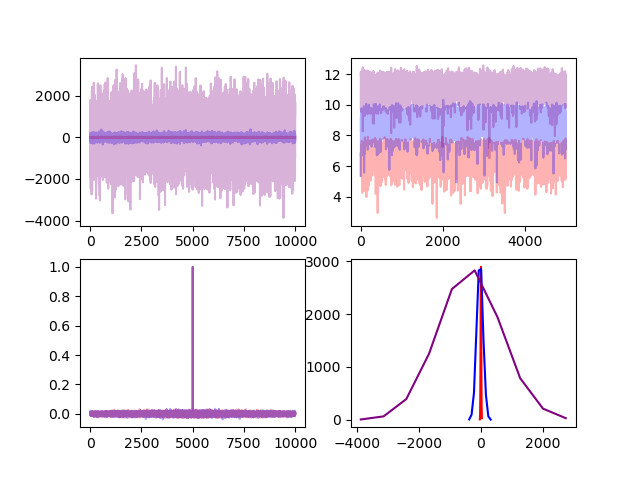
\includegraphics[width=10cm]{noise.png}
\caption{(UL) A stochastic process drawn from a normal distribution with variance 1,10,1000. (UR) Power spectral density of the three stochastic processes (LL) Autocorrelation function for the three processes. (LR) Empirical amplitude distribution for the three processes.}
\end{figure}

Recall that the Fourier transform of the autocorrelation function of a signal is equivalent to its power spectral density (PSD). That is, the autocorrelation function and the PSD form a Fourier pair. At the same time, we know that Fourier transform of a delta function is a flat function (this has very important consequences in quantum mechanics and is related to the Heisenberg uncertainty principle). Therefore, if we have a stochastic process with a flat PSD, then its autocorrelation function is a delta function and it is "delta-correlated". This means that every time step is completely uncorrelated with every other time step.

At this point I want to take note of the terminology. The term white noise refers to a property of the PSD and therefore the shape of the autocorrelation function. It refers to the delta-correlated-ness of the proces. It does not refer to say, the distribution the process is sampled from (in the case that the process has stationary statistics). For example, if the stochastic process is simply a sequence of samples from a Gaussian (normal) distribution, but the samples are drawn i.i.d, the PSD will be flat and the autocorrelation function will be a delta-function. Here, the Gaussian is simply the amplitude distribution of the process and there are many such distributions will all can parameterize white stochastic processes. 




\end{document}